\documentclass{standalone}
\usepackage{tikz}
\usepackage{ctex,siunitx}
\setCJKmainfont{Noto Serif CJK SC}
\usepackage{tkz-euclide}
\usepackage{amsmath}
\usetikzlibrary{patterns, calc,3d}
\usetikzlibrary {decorations.pathmorphing,decorations.pathreplacing,decorations.shapes}
\begin{document}
\small
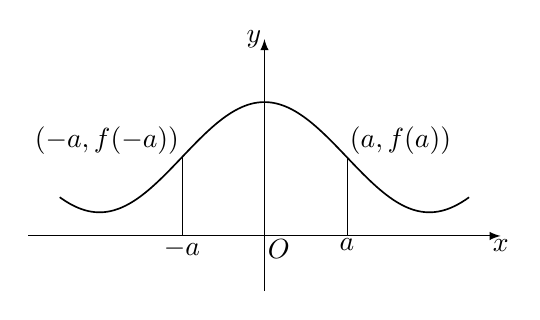
\begin{tikzpicture}[>=latex,scale=1.0,inner sep=1pt]
  \draw[->](-3,0)--(3,0)node[below]{$x$};
  \draw[->](0,-0.7)--(0,2.5)node[left]{$y$};
  \node at (0,0)[below right]{$O$};
  \draw[semithick,samples=200,domain=-2.6:2.6]plot(\x,{1+0.7*cos(1.5*\x r)});
  \draw[very thin](pi/3,{1+0.7*cos(pi/2 r)})node[above right]{$(a,f(a))$}--(pi/3,0)node[below]{$a$};
  \draw[very thin](-pi/3,{1+0.7*cos(-pi/2 r)})node[above left]{$(-a,f(-a))$}--(-pi/3,0)node[below]{$-a$};
\end{tikzpicture}
\end{document}